\PassOptionsToPackage{quiet}{fontspec} 
\documentclass{ctexart}
\usepackage{lipsum}
\usepackage{xcolor,listings}
\usepackage{graphicx}
\graphicspath{{imgs/}}
% \ctexset{section={format+=\raggedright}}
\lstset{
    showstringspaces=false,
    frame=single,
    numbers=left,
    numberstyle=\color{darkgray},
    backgroundcolor=\color{white},
    keywordstyle=\color{blue},
    commentstyle=\it\color[RGB]{0,100,0},
    stringstyle=\sl\color{red},
}
\begin{document}
\title{数字图像处理基础-图书ISBN号字符识别}
\author{覃梓鑫(软工2003-20202005175)}
\date{\today}
\maketitle
\tableofcontents
\newpage
\section{概述}
\noindent
\textbf{设计目的:}\\
\textbf{内容:}\\
\textbf{运行环境:}
Windows10 + Python 3.10.6\\
所需 Python 第三方库如下:
\begin{itemize}
    \item 略
\end{itemize}
\noindent
\textbf{开发工具:}%不用加多余的\\
\begin{itemize}
    \item 操作系统 Windows 10 21H2
    \item 集成开发环境 Visual Studio Code 1.73.1
    \item 文档编写工具 TeXworks 0.6.6
    \item 编程语言 Python 3.10.6
    % \item 版本管理工具 git 2.29.0
    \item 编码格式 UTF8
\end{itemize}

\section{整体设计}
\section{具体实现}
\textit{为了表述的方便,该节按照模块进行分节,并在每个模块内部分别描述其具体必要的程序框图、数学模型、核心程序与处理过程图片。}
\subsection{灰度化}
根据课件(第11章-P38页-4彩色平衡)内容可知,彩色图像数字化后,景物颜色会偏移真实颜色,导致三基色不平衡。这里采用白平衡法计算灰度,即使用公式:%不需要\\
\[I(x,y)=0.299\cdot f_R(x,y)+0.587\cdot f_G(x,y)+0.114\cdot f_B(x,y)\] %不需要\\
但是如果直接使用Python迭代来处理上述过程,非常缓慢。所以考虑用\textbf{矩阵运算优化}。我们知道,向量内积的计算结果是实数,故有:
\[(R,G,B)\cdot(0.299,0.587,0.114)=0.299R+0.587G+0.114B\]
因此,考虑用向量内积,直接调用底层依托 C++ 实现的 numpy 的向量运算 `dot` 函数,一来 C++ 比 Python 快,二来矩阵运算比迭代快,这样能起到不小的常数优化作用。在下文的其他具体实现里也会反复用到类似的思路。因此,核心代码如下:
\begin{lstlisting}[language=python]
import numpy as np
def toGrey(img):
    rd = img.shape[2]  # 可能是3/4(png有alpha通道)
    line = [0.299, 0.587, 0.114, 0][:rd]
    arr = [line for i in range(rd)]
    trans = np.array(arr).transpose()  # 矩阵转置
    img2 = np.dot(img, trans).astype(img.dtype)
    return img2
\end{lstlisting}
运行效果如下:
\begin{figure}[htbp]
    \centering
    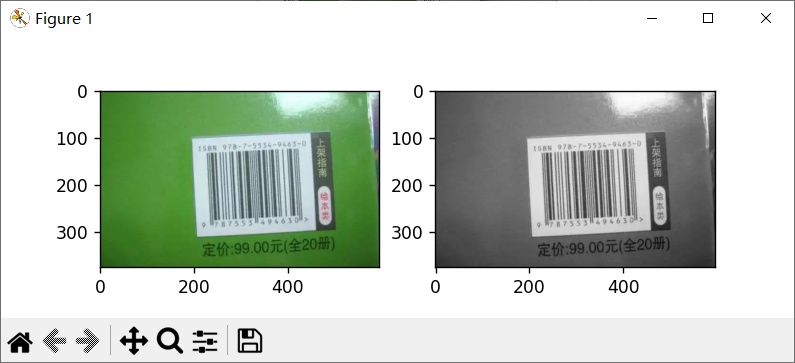
\includegraphics[height=120pt]{sample_toGrey}
    \caption{灰度化效果展示}
\end{figure}
\section{实验结果及分析}
\section{总结与体会}
\section{致谢}
\section{参考文献}
\section{附录}
\end{document}